\section{\LaTeX{} Typesetting Examples}

\subsection{\LaTeX{} Basics}

% This is not a real section; it's just here to show examples of how to format various components. Remove it before submitting!

\begin{itemize}
    \item Here's a regular bulleted list item.
    \item And another.
\end{itemize}

Here's a \href{https://datascience.ucsd.edu}{hyperlink}. If you want to use a numbered list, you can experiment with:

\begin{enumerate}
    \item This.
    \item This.
    \item And this.
\end{enumerate}

Here's how you might include a snippet of actual code:

\begin{verbatim}
# If you want to use syntax highlighting, look into the minted package.
def f(x):
    return 2 * x + 3
\end{verbatim}

Here's how you might format a single equation:

$$\int_{-\infty}^\infty f_X(x)dx = 1$$

And a chain of equations:

\begin{align*}
    \frac{1}{n}\sum_{i = 1}^n (x_i - \bar{x})^2 &= \frac{1}{n}\sum_{i = 1}^n (x_i^2 - 2x_i\bar{x} + \bar{x}^2)
    \\ &= \frac{1}{n}\sum_{i = 1}^n x_i^2 - \frac{2}{n}\bar{x}\sum_{i = 1}^n x_i + \frac{\bar{x}^2}{n}\sum_{i = 1}^n 1
    \\ &= \frac{1}{n}\sum_{i = 1}^n x_i^2 - 2\bar{x}^2 + \bar{x}^2
    \\ &= \frac{1}{n}\sum_{i = 1}^n x_i^2 - \bar{x}^2
\end{align*}


\subsection{Figure Examples}

Here are some example figures. 
Figure \ref{fig:somefig1} presents a scatter plot.

\begin{figure}[htbp]
\centering
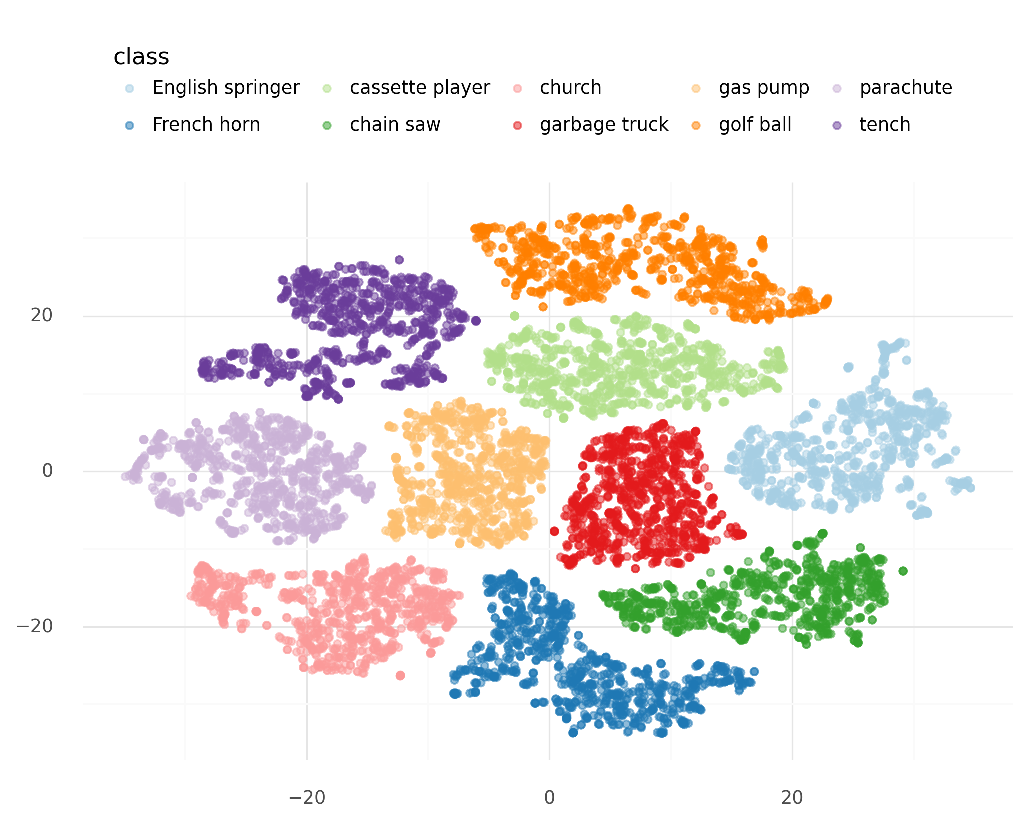
\includegraphics[width=.65\linewidth]{figure/somefig1.pdf}
\caption{Yes, put a few words or sentences here explaining what is in the figure.}
\label{fig:somefig1}
\end{figure}

Figure \ref{fig:someotherfigs} presents some summaries of the performance of our model.
The left panel of Figure \ref{fig:someotherfigs} presents something.
The right panel of Figure \ref{fig:someotherfigs} presents some other things.

\begin{figure}[htbp]
\begin{minipage}{0.53\linewidth}
  \centering
  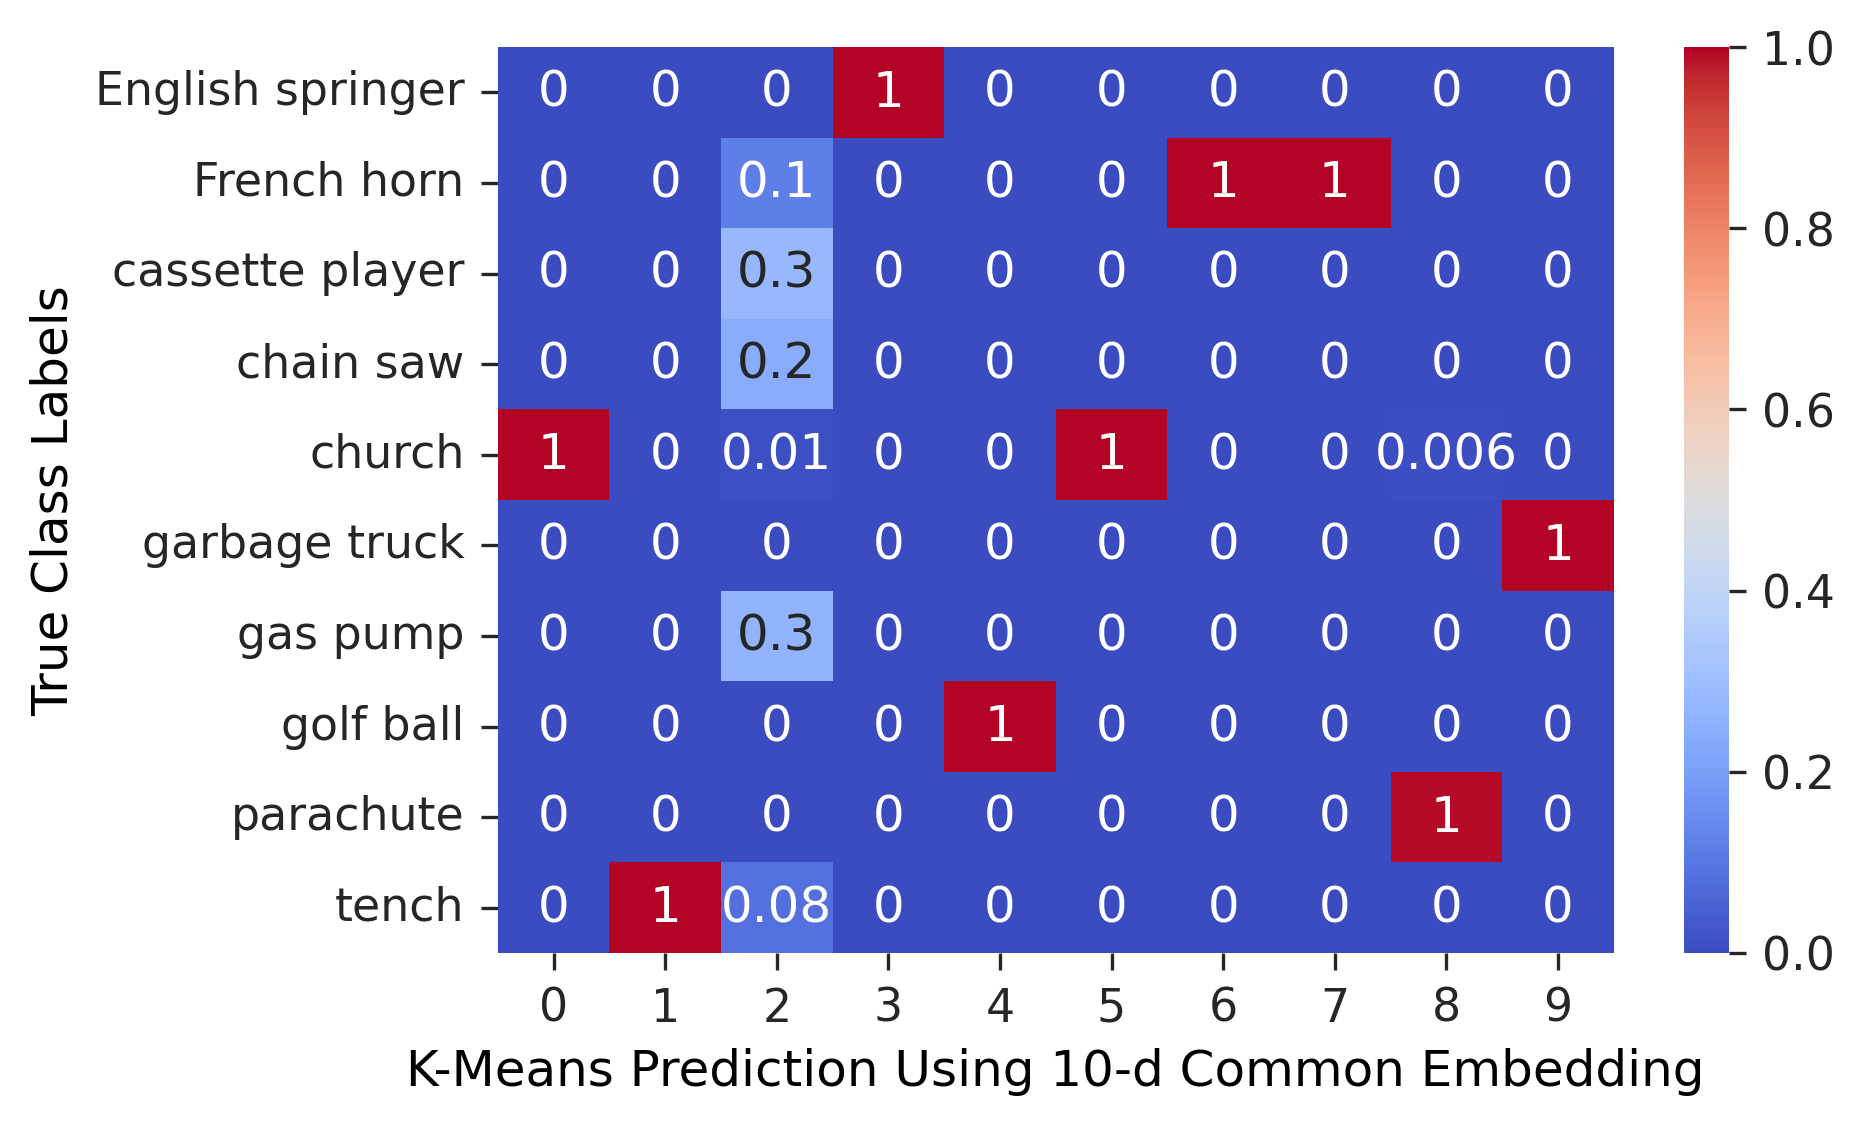
\includegraphics[width=\linewidth]{figure/somefig2.png}
\end{minipage}
\begin{minipage}{0.42\linewidth}
  \centering
  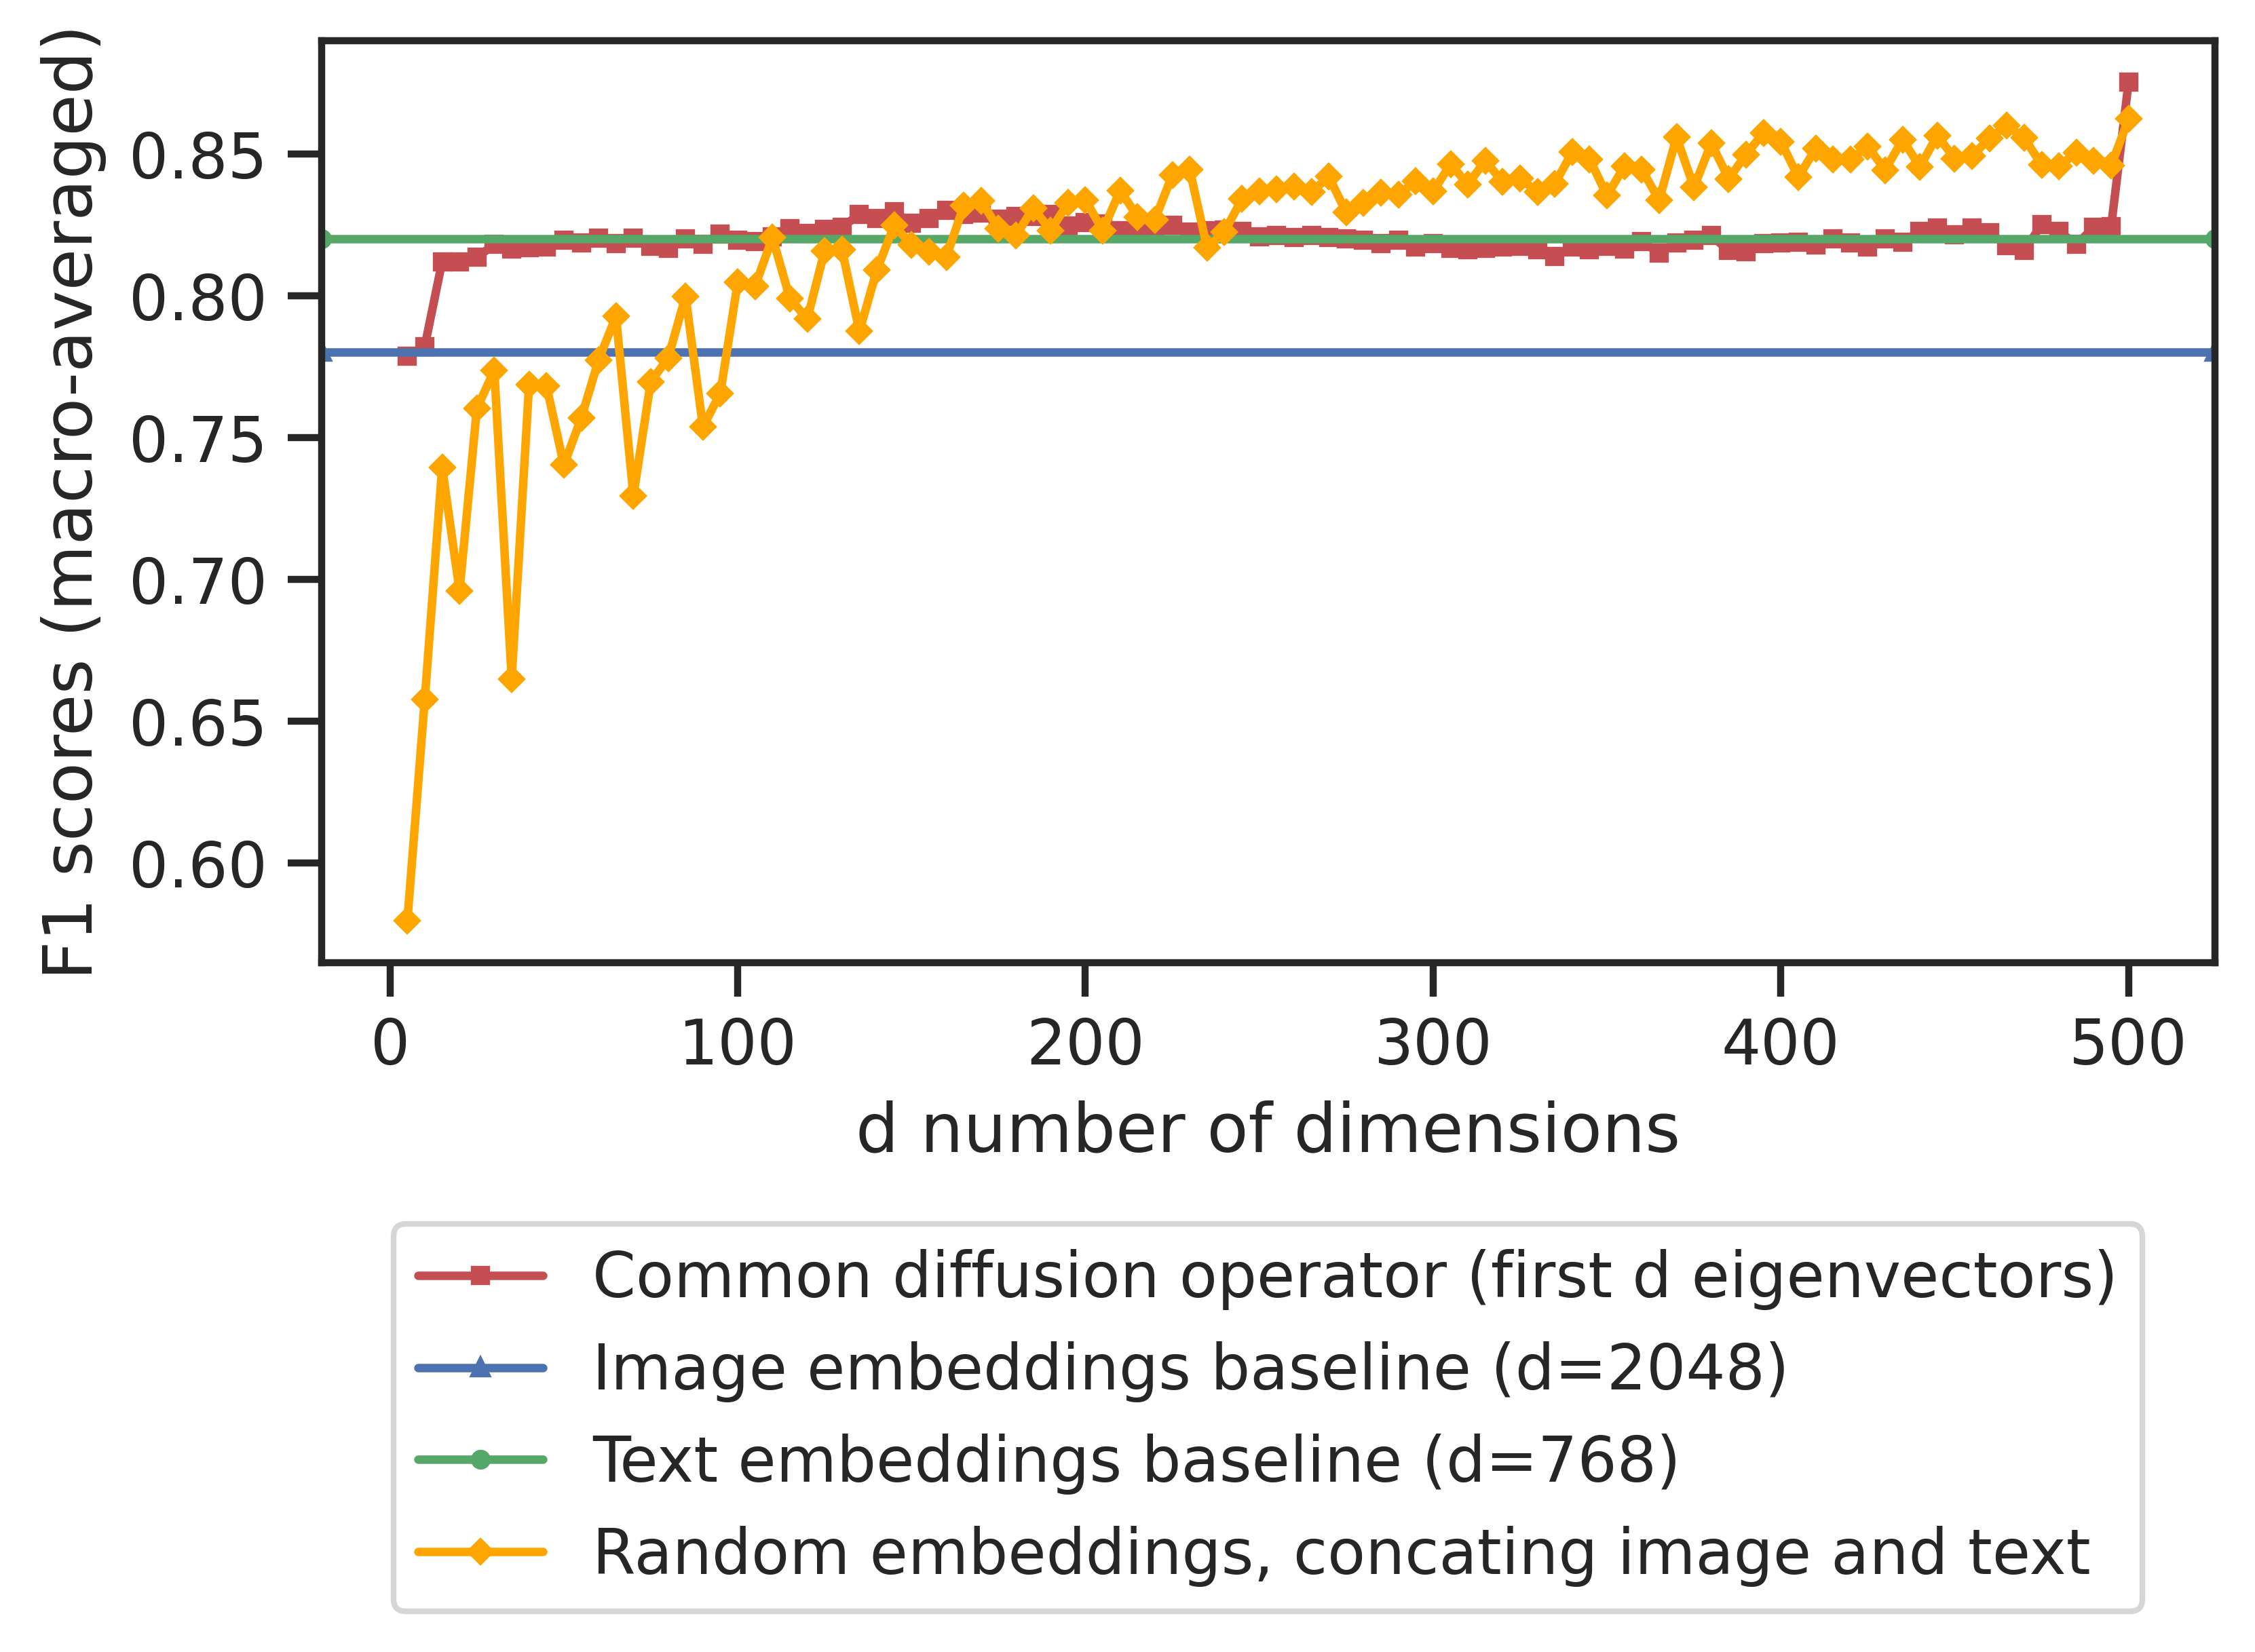
\includegraphics[width=\linewidth]{figure/somefig3.png}
\end{minipage}
\caption{You can put figures side-by-side as well.}
\label{fig:someotherfigs}
\end{figure}


\subsection{Table Examples}

Table \ref{tab:sometab1} presents some summary of the data.

\begin{table}[htbp]
\caption{Some Table Caption}
\label{tab:sometab1}
\resizebox{0.4\linewidth}{!}{\centering
\begin{tabular}{lll}
\toprule
\multicolumn{2}{c}{Part}                   \\
\cmidrule(r){1-2}
Name     & Description     & Size ($\mu$m) \\
\midrule
Dendrite & Input terminal  & $\sim$100     \\
Axon     & Output terminal & $\sim$10      \\
Soma     & Cell body       & up to $10^6$  \\
\bottomrule
\end{tabular}}
\end{table}

Table \ref{tab:sometab2} presents some summaries of the performance of our model.

\begin{table}[htbp]
\caption{Some Other Table Caption}
\label{tab:sometab2}
\resizebox{0.9\linewidth}{!}{\centering
\begin{tabular}{l|lcccccc}
\toprule
Method & Modality & Edit distance & BLEU & METEOR & Precision & Recall & F1 \\ \midrule
PDF                  & All      & 0.255 & 65.8 & 82.1 & 77.1 & 81.4 & 79.2 \\ \hline
GROBID               & All      & 0.312 & 55.6 & 71.9 & 74.0 & 72.1 & 73.0 \\ \cline{2-8}
                     &Tables    & 0.626 & 25.1 & 64.5 & 61.4 & 80.7 & 69.7 \\
+ LaTeX OCR %
                     & Plain text &0.363 & 57.4 & 69.2 & 82.1 & 70.5 & 75.9 \\
                     & Math     & 0.727 & 0.3 & 5.0 & 11.0 & 8.6 & 9.7 \\ \hline
\multirow{4}{*}{Nougat base (350M$^\ast$)} & All & \bf 0.071 & \bf 89.1 & \bf 93.0 & 93.5 & \bf 92.8 & \bf 93.1 \\ \cline{2-8}
                     & Tables     & 0.211 & 69.7 & 79.1 & 75.4 & 80.7 & 78.0 \\ 
                     & Plain text & 0.058         & 91.2 & 94.6   & 96.2      & 95.3   & 95.7 \\
                     & Math       & 0.128         & 56.9 & 75.4   & 76.5      & 76.6   & 76.5 \\ \bottomrule
\end{tabular}}
\end{table}

\subsection{Equations and Algorithms Examples}

Algorithm \ref{alg:fuzzyKmeans} implements Fuzzy K-means.

\begin{algorithm}
\caption{Fuzzy K-means clustering algorithm}
\label{alg:fuzzyKmeans}
\begin{enumerate}
    \item Choose primary centroids $v_{k}$
    \item Compute the membership degree of all feature vectors in all clusters
    \begin{equation}
    u_{ki}  = \frac{1}{ \sum_{j=1}^K ( \frac{D^{2}(x_{i} - v_{k})}{D^{2}(x_{i} - v_{j})})^\frac{2} 
    {m-1}}
    \label{eq:kmeans}
    \end{equation}
\end{enumerate}
\end{algorithm}

Algorithm \ref{alg:net} calculates net activation.


\begin{algorithm}
\caption{Computing Net Activation}
\label{alg:net}
% \DontPrintSemicolon
% \LinesNumbered
\KwIn{$x_1, \ldots, x_n, w_1, \ldots, w_n$}
\KwOut{$y$, the net activation}
$y\leftarrow 0$\;
\For{$i\leftarrow 1$ \KwTo $n$}{
$y \leftarrow y + w_i*x_i$\;
}
\end{algorithm}

In Variational Autoencoder (VAE), we directly maximize the Evidence Lower Bound (ELBO) using the following Equations \ref{eq:bla}--\ref{eq:blablabla}.
\begin{align}
  \mathbb{E}_{q_{\boldsymbol{\phi}}(\boldsymbol{z}\mid\boldsymbol{x})}\left[\log\frac{p(\boldsymbol{x}, \boldsymbol{z})}{q_{\boldsymbol{\phi}}(\boldsymbol{z}\mid\boldsymbol{x})}\right]
  &= \mathbb{E}_{q_{\boldsymbol{\phi}}(\boldsymbol{z}\mid\boldsymbol{x})}\left[\log\frac{p_{\boldsymbol{\theta}}(\boldsymbol{x}\mid\boldsymbol{z})p(\boldsymbol{z})}{q_{\boldsymbol{\phi}}(\boldsymbol{z}\mid\boldsymbol{x})}\right] \label{eq:bla} \\
  &= \mathbb{E}_{q_{\boldsymbol{\phi}}(\boldsymbol{z}\mid\boldsymbol{x})}\left[\log p_{\boldsymbol{\theta}}(\boldsymbol{x}\mid\boldsymbol{z})\right] + \mathbb{E}_{q_{\boldsymbol{\phi}}(\boldsymbol{z}\mid\boldsymbol{x})}\left[\log\frac{p(\boldsymbol{z})}{q_{\boldsymbol{\phi}}(\boldsymbol{z}\mid\boldsymbol{x})}\right] \label{eq:blabla} \\
  &= \underbrace{\mathbb{E}_{q_{\boldsymbol{\phi}}(\boldsymbol{z}\mid\boldsymbol{x})}\left[\log p_{\boldsymbol{\theta}}(\boldsymbol{x}\mid\boldsymbol{z})\right]}_\text{reconstruction term} - \underbrace{\mathcal{D}_{\text{KL}}(q_{\boldsymbol{\phi}}(\boldsymbol{z}\mid\boldsymbol{x}) \mid\mid p(\boldsymbol{z}))}_\text{prior matching term} \label{eq:blablabla}
\end{align}

\subsection{Inline Citation Examples}

Citation in text (no parentheses): use \texttt{{\textbackslash}cite\{citekey\}}. 
For example, \cite{breiman2011}, \cite{devlin2019bert}.

Citation in parentheses: use \texttt{{\textbackslash}citep\{citekey\}}. 
For example: \citep{vaswani2023attention}, \citep{karras2019stylebased}.
